\section*{Приложения}
\addcontentsline{toc}{section}{Приложения}

\counterwithin{figure}{subsection}
\counterwithin{table}{subsection}
\counterwithin{equation}{subsection}

\renewcommand{\thesubsection}{\Alph{subsection}}

\subsection{Результаты экспериментов в модели Манна}\label{appendix:a}

\begin{figure}[h]
	\centering
	\hspace{-20mm}
	\begin{subfigure}[t]{0.4\textwidth}
		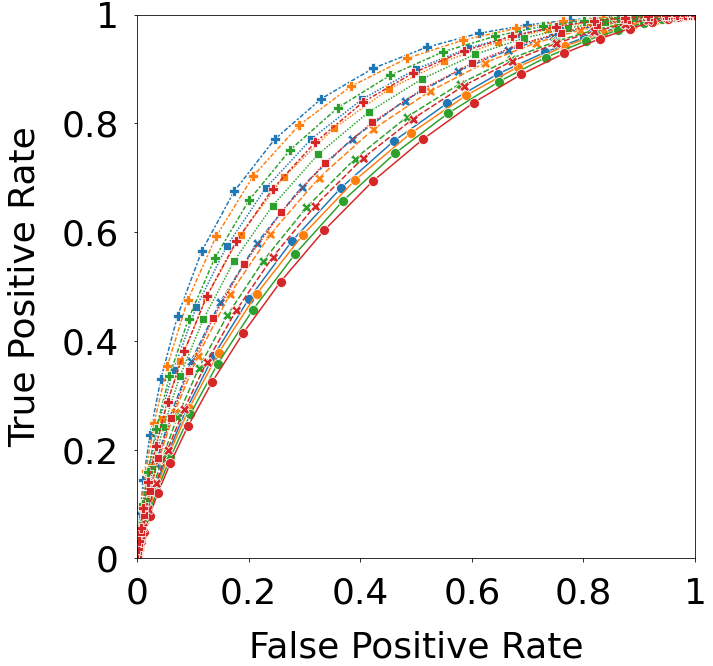
\includegraphics[height=\textwidth]{manna_roc_255} 
		\caption{ROC-кривые}
	\end{subfigure}
	\hspace*{10mm}
	\begin{subfigure}[t]{0.4\textwidth}
		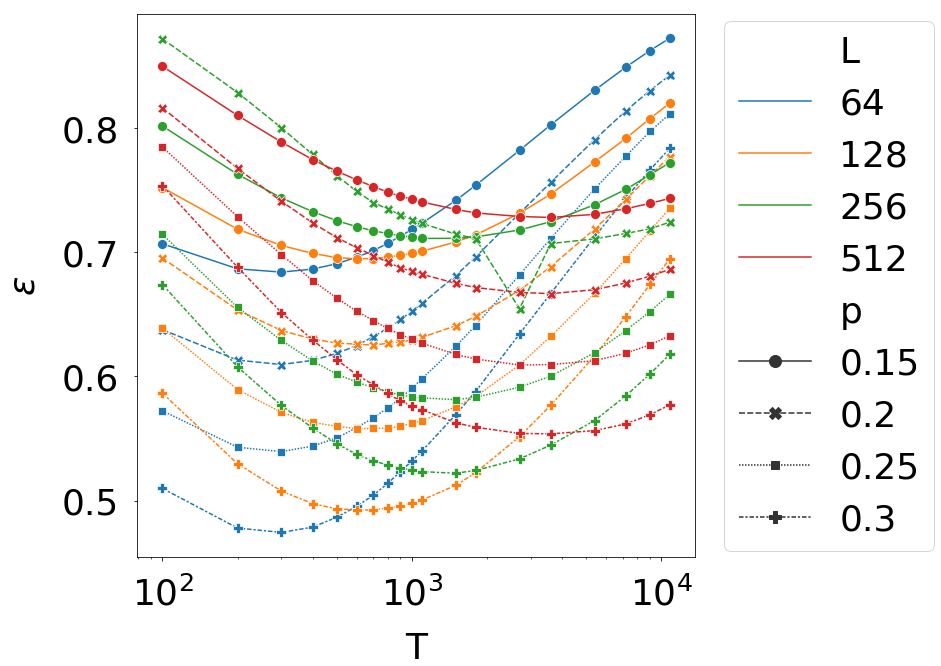
\includegraphics[height=\textwidth]{manna_t_255} 
		\caption{Качество прогноза}
	\end{subfigure}
	\caption{Качество прогноза в зависимости от $T$ для разных констант $p$ и фиксированного параметра $\gamma=2.55$ в модели Манна}
\end{figure}

\begin{figure}[h]
	\centering
	\hspace{-20mm}
	\begin{subfigure}[t]{0.4\textwidth}
		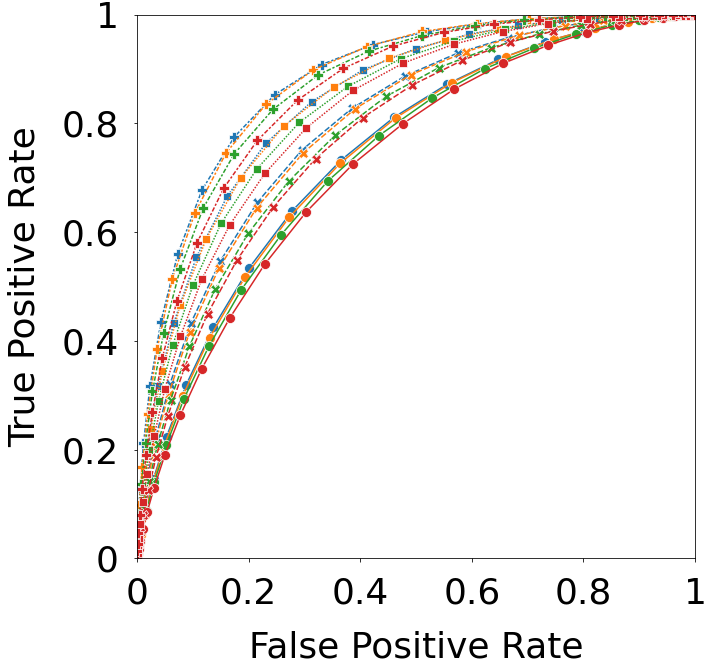
\includegraphics[height=\textwidth]{manna_roc_260} 
		\caption{ROC-кривые}
	\end{subfigure}
	\hspace*{10mm}
	\begin{subfigure}[t]{0.4\textwidth}
		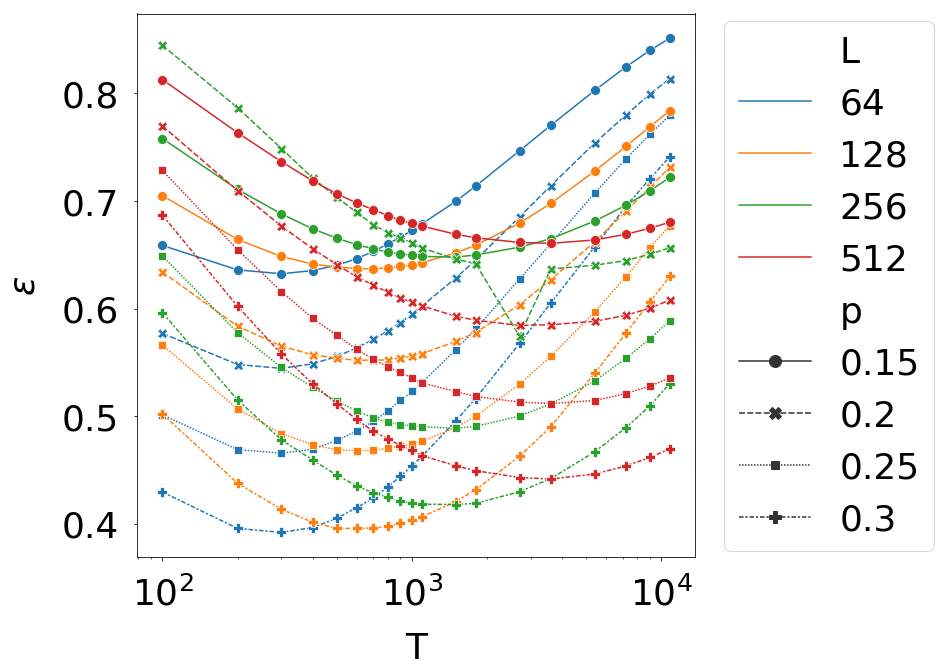
\includegraphics[height=\textwidth]{manna_t_260} 
		\caption{Качество прогноза}
	\end{subfigure}
	\caption{Качество прогноза в зависимости от $T$ для разных констант $p$ и фиксированного параметра $\gamma=2.6$ в модели Манна}
\end{figure}

\begin{figure}[h]
	\centering
	\hspace{-20mm}
	\begin{subfigure}[t]{0.4\textwidth}
		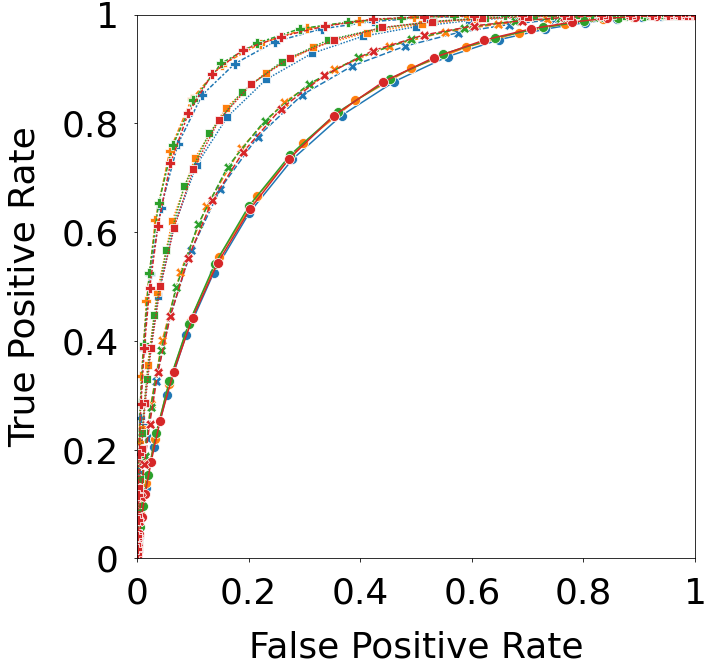
\includegraphics[height=\textwidth]{manna_roc_267} 
		\caption{ROC-кривые}
	\end{subfigure}
	\hspace*{10mm}
	\begin{subfigure}[t]{0.4\textwidth}
		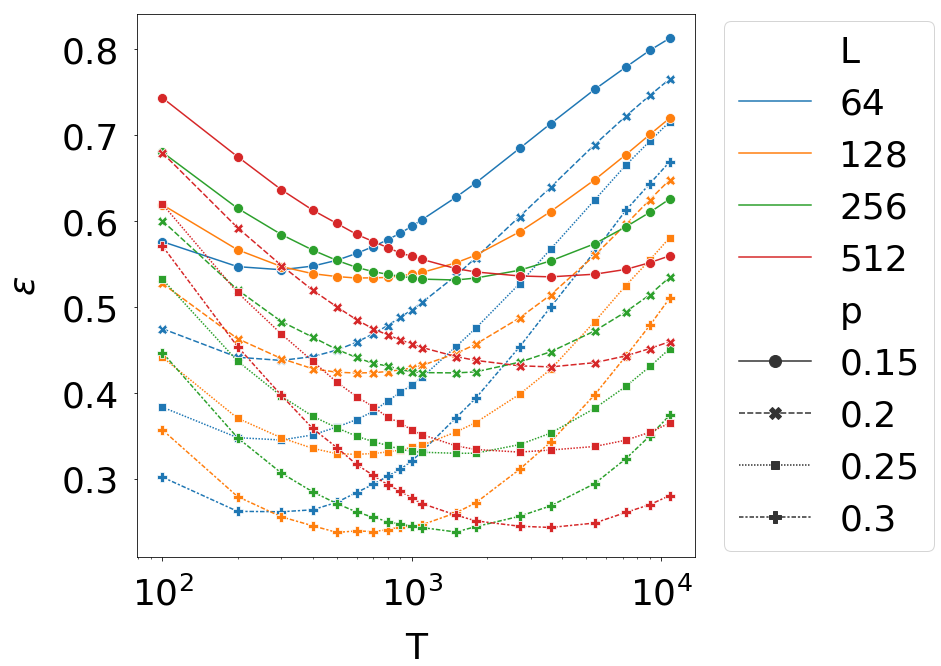
\includegraphics[height=\textwidth]{manna_t_267} 
		\caption{Качество прогноза}
	\end{subfigure}
	\caption{Качество прогноза в зависимости от $T$ для разных констант $p$ и фиксированного параметра $\gamma=2.67$ в модели Манна}
\end{figure}

\begin{figure}[h]
	\centering
	\hspace{-20mm}
	\begin{subfigure}[t]{0.4\textwidth}
		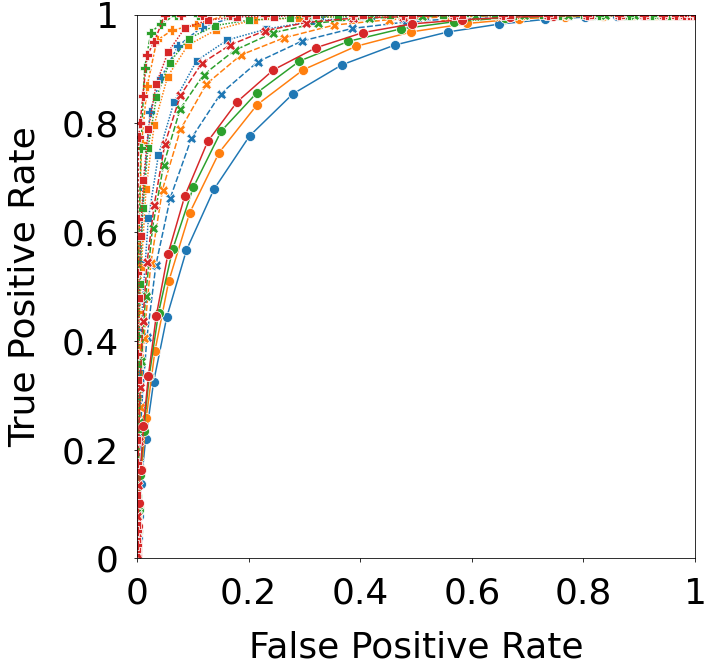
\includegraphics[height=\textwidth]{manna_roc_275} 
		\caption{ROC-кривые}
	\end{subfigure}
	\hspace*{10mm}
	\begin{subfigure}[t]{0.4\textwidth}
		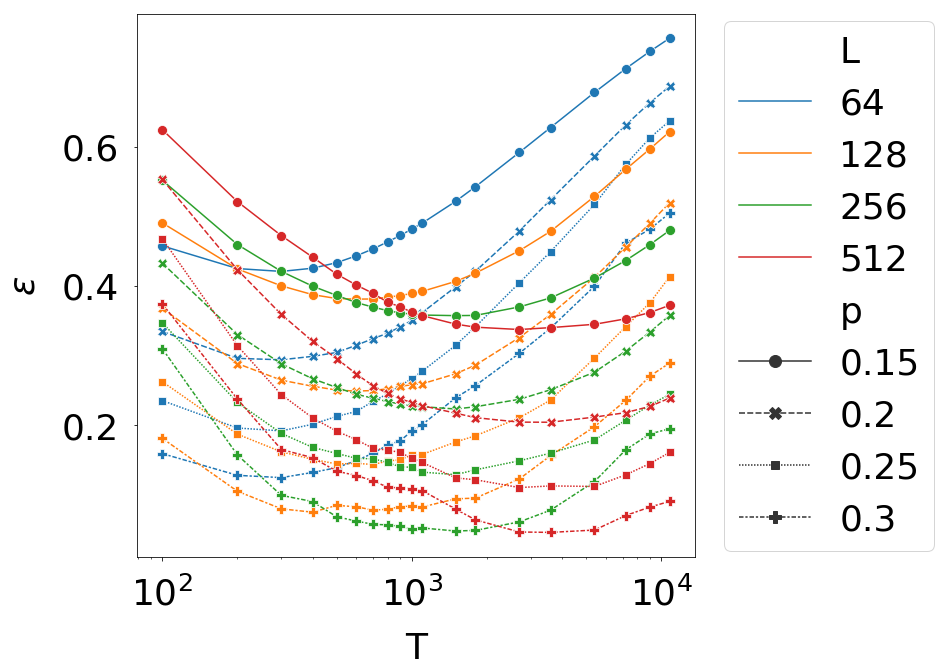
\includegraphics[height=\textwidth]{manna_t_275} 
		\caption{Качество прогноза}
	\end{subfigure}
	\caption{Качество прогноза в зависимости от $T$ для разных констант $p$ и фиксированного параметра $\gamma=2.75$ в модели Манна}
\end{figure}

\newpage
\clearpage

\subsection{Результаты экспериментов в модели БТВ}\label{appendix:b}

\begin{figure}[h]
	\centering
	\hspace{-20mm}
	\begin{subfigure}[t]{0.4\textwidth}
		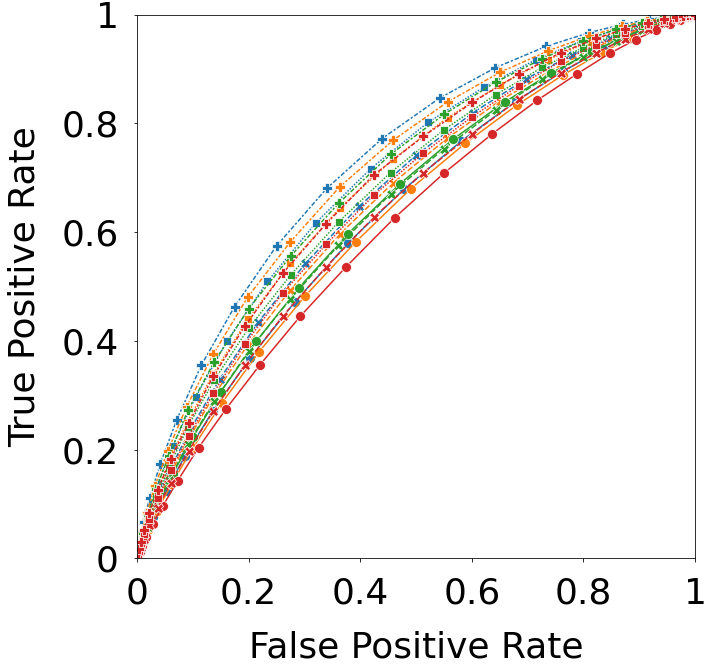
\includegraphics[height=\textwidth]{btw_roc_280} 
		\caption{ROC-кривые}
	\end{subfigure}
	\hspace*{10mm}
	\begin{subfigure}[t]{0.4\textwidth}
		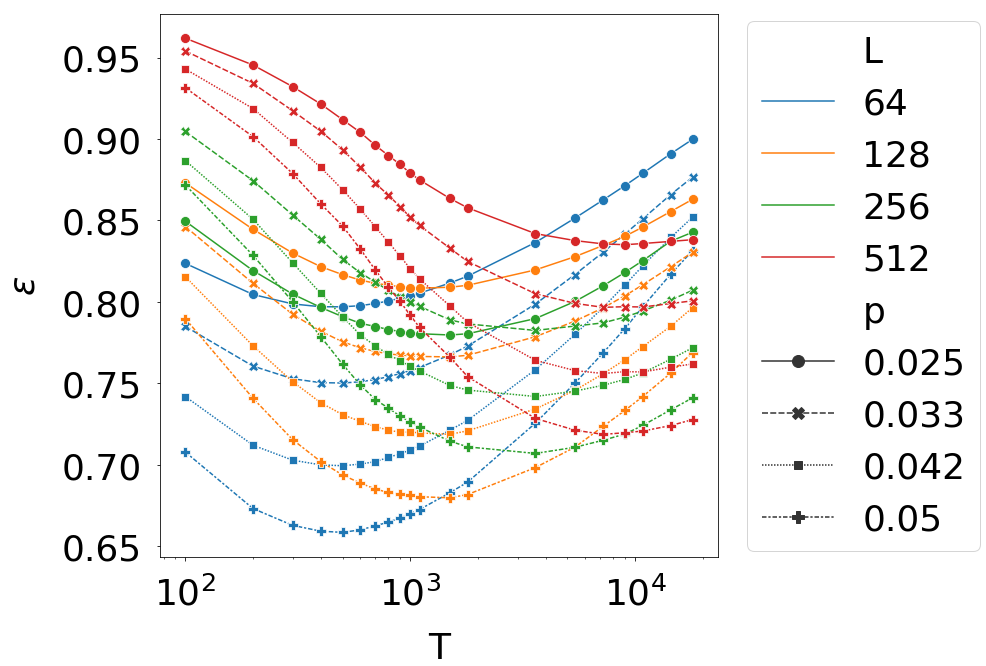
\includegraphics[height=\textwidth]{btw_t_280} 
		\caption{Качество прогноза}
	\end{subfigure}
	\caption{Качество прогноза в зависимости от $T$ для разных констант $p$ и фиксированного параметра $\gamma=2.8$ в модели БТВ}
\end{figure}

\begin{figure}[h]
	\centering
	\hspace{-20mm}
	\begin{subfigure}[t]{0.4\textwidth}
		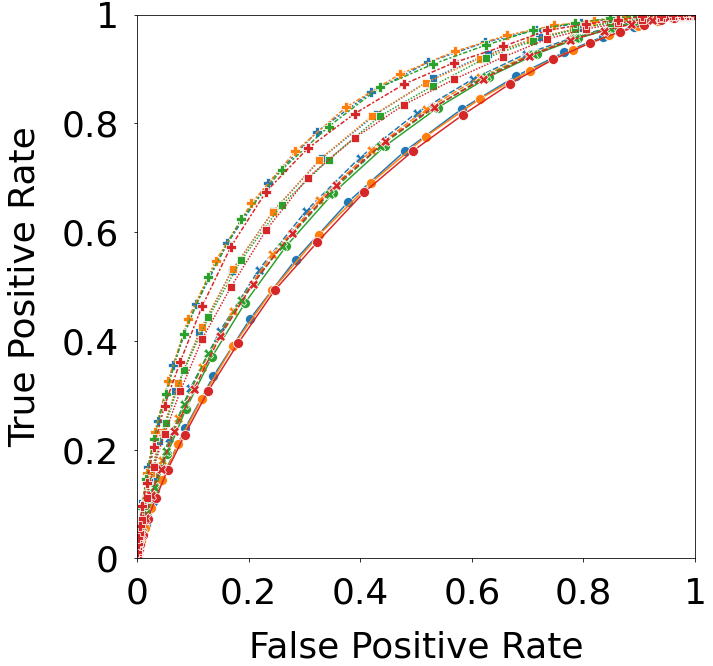
\includegraphics[height=\textwidth]{btw_roc_290} 
		\caption{ROC-кривые}
	\end{subfigure}
	\hspace*{10mm}
	\begin{subfigure}[t]{0.4\textwidth}
		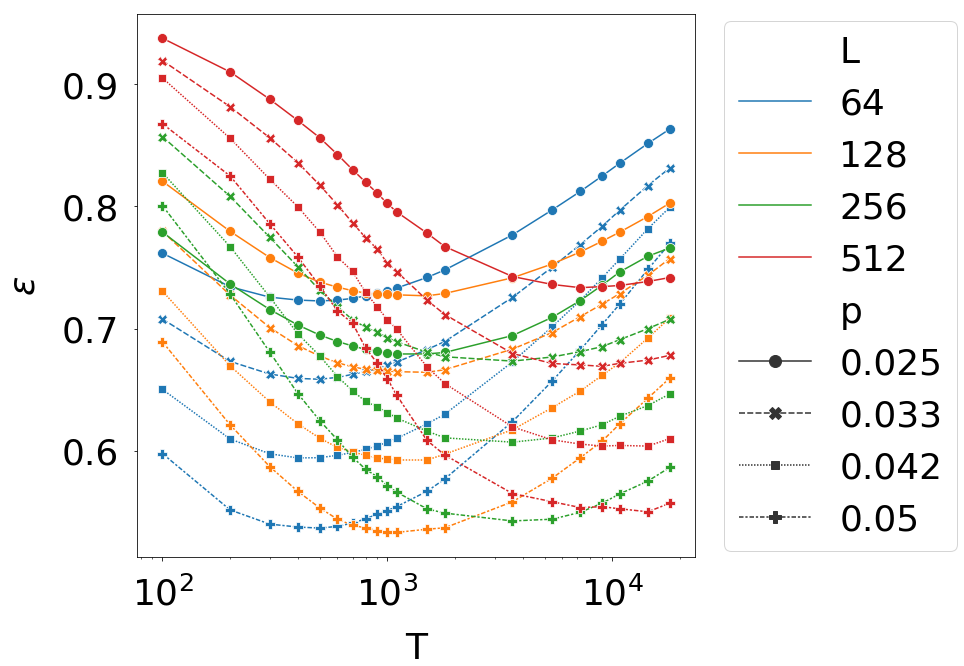
\includegraphics[height=\textwidth]{btw_t_290} 
		\caption{Качество прогноза}
	\end{subfigure}
	\caption{Качество прогноза в зависимости от $T$ для разных констант $p$ и фиксированного параметра $\gamma=2.9$ в модели БТВ}
\end{figure}

\begin{figure}[h]
	\centering
	\hspace{-20mm}
	\begin{subfigure}[t]{0.4\textwidth}
		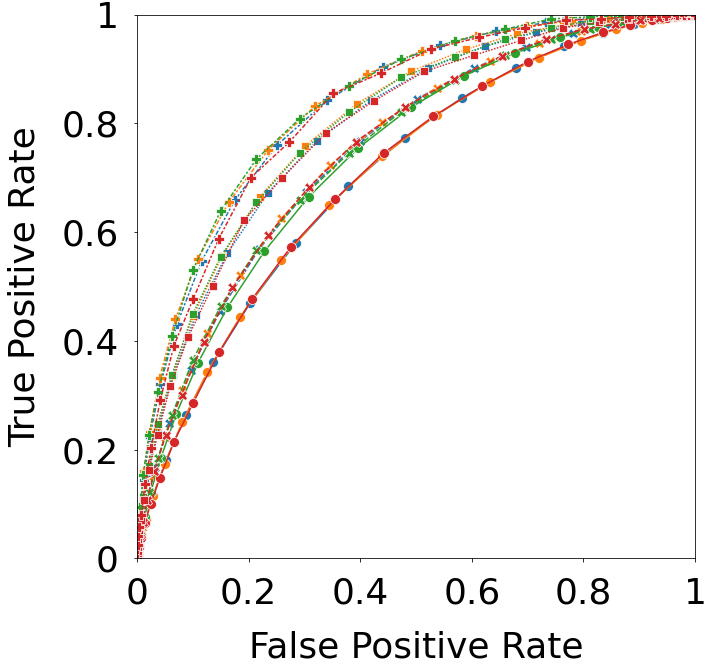
\includegraphics[height=\textwidth]{btw_roc_293} 
		\caption{ROC-кривые}
	\end{subfigure}
	\hspace*{10mm}
	\begin{subfigure}[t]{0.4\textwidth}
		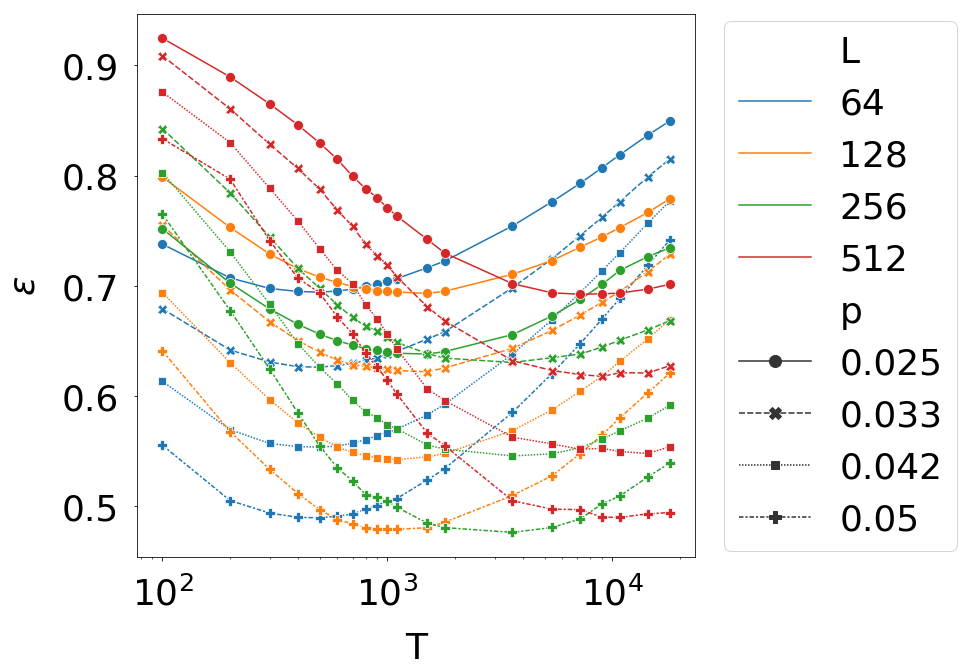
\includegraphics[height=\textwidth]{btw_t_293} 
		\caption{Качество прогноза}
	\end{subfigure}
	\caption{Качество прогноза в зависимости от $T$ для разных констант $p$ и фиксированного параметра $\gamma=2.93$ в модели БТВ}
\end{figure}

\begin{figure}[h]
	\centering
	\hspace{-20mm}
	\begin{subfigure}[t]{0.4\textwidth}
		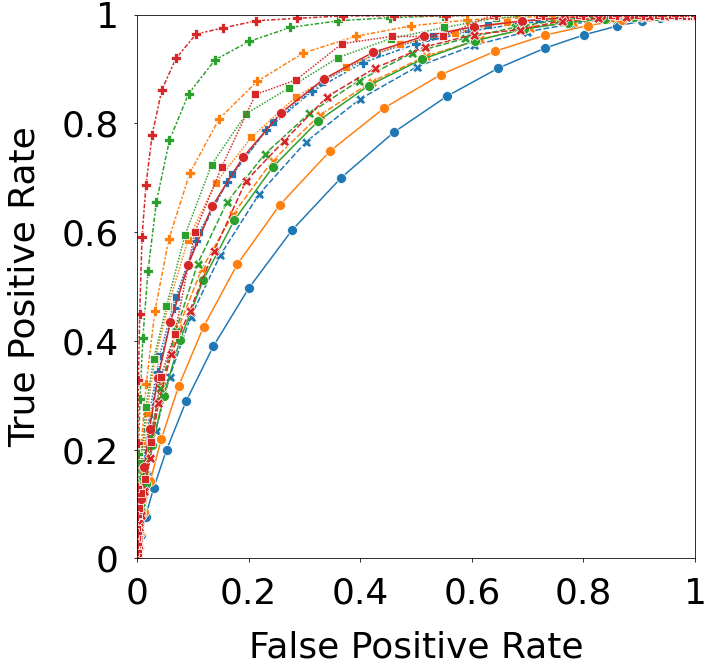
\includegraphics[height=\textwidth]{btw_roc_300} 
		\caption{ROC-кривые}
	\end{subfigure}
	\hspace*{10mm}
	\begin{subfigure}[t]{0.4\textwidth}
		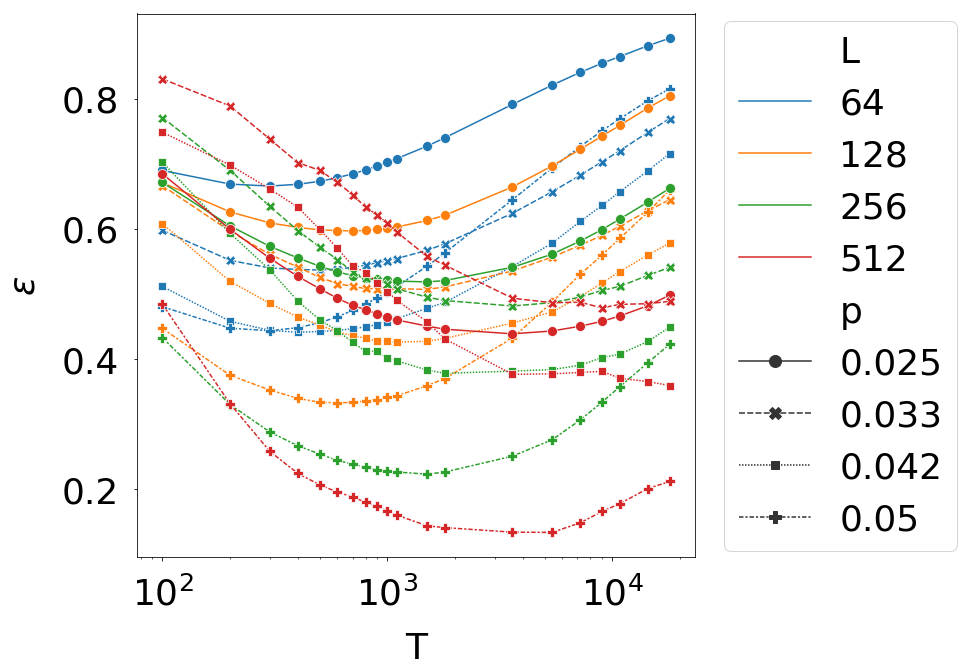
\includegraphics[height=\textwidth]{btw_t_300} 
		\caption{Качество прогноза}
	\end{subfigure}
	\caption{Качество прогноза в зависимости от $T$ для разных констант $p$ и фиксированного параметра $\gamma=3$ в модели БТВ}
\end{figure}

\newpage
\clearpage

\subsection{Количество прогнозируемых событий}\label{appendix:c}
\begin{table}[h]
	\caption{Количество прогнозируемых событий в модели БТВ для заданных констант $p$ и размеров решеток $L$}
	\begin{tabular}{cc}
		$\gamma = 2.93$ & $\gamma = 3$ \\
		\begin{tabular}{l|rrrr}
			\toprule
			p &     64  &    128 &    256 &   512 \\
			\midrule
			0.025 &  173167 &  61170 &  23634 &  9544 \\
			0.033 &   75863 &  24653 &   9117 &  3684 \\
			0.042 &   30507 &   9244 &   3201 &  1265 \\
			0.050 &   13563 &   3779 &   1300 &   528 \\
			\bottomrule
		\end{tabular} &
		\begin{tabular}{l|rrrr}
			\toprule
			p &    64  &    128 &   256 &   512 \\
			\midrule
			0.025 &  72492 &  19542 &  5910 &  1841 \\
			0.033 &  24616 &   5706 &  1531 &   458 \\
			0.042 &   7155 &   1403 &   347 &    75 \\
			0.050 &   2346 &    366 &    82 &    10 \\
			\bottomrule
		\end{tabular}
	\end{tabular}
\end{table}

\begin{table}[h]
	\caption{Количество прогнозируемых событий в модели Манна для заданных констант $p$ и размеров решеток $L$}
	\begin{tabular}{cc}
		$\gamma = 2.67$ & $\gamma = 2.75$ \\
		\begin{tabular}{l|rrrr}
			\toprule
			p &     64  &    128 &    256 &    512 \\
			\midrule
			0.15 &  108114 &  70910 &  47169 &  32008 \\
			0.20 &   43514 &  30106 &  21248 &  15164 \\
			0.25 &   16146 &  11885 &   9042 &   6802 \\
			0.30 &    5253 &   4116 &   3487 &   2879 \\
			\bottomrule
		\end{tabular}
		&
		\begin{tabular}{lrrrr}
			\toprule
			p &    64  &    128 &    256 &   512 \\
			\midrule
			0.15 &  36614 &  20603 &  11990 &  7117 \\
			0.20 &   8569 &   4598 &   2787 &  1674 \\
			0.25 &   1554 &    839 &    507 &   299 \\
			0.30 &    225 &    106 &     62 &    40 \\
			\bottomrule
		\end{tabular}
	\end{tabular}
\end{table}

\newpage
\clearpage

\subsection{Распределение событий в модели Манна}\label{appendix:d}

\begin{figure}[h]
	\centering
	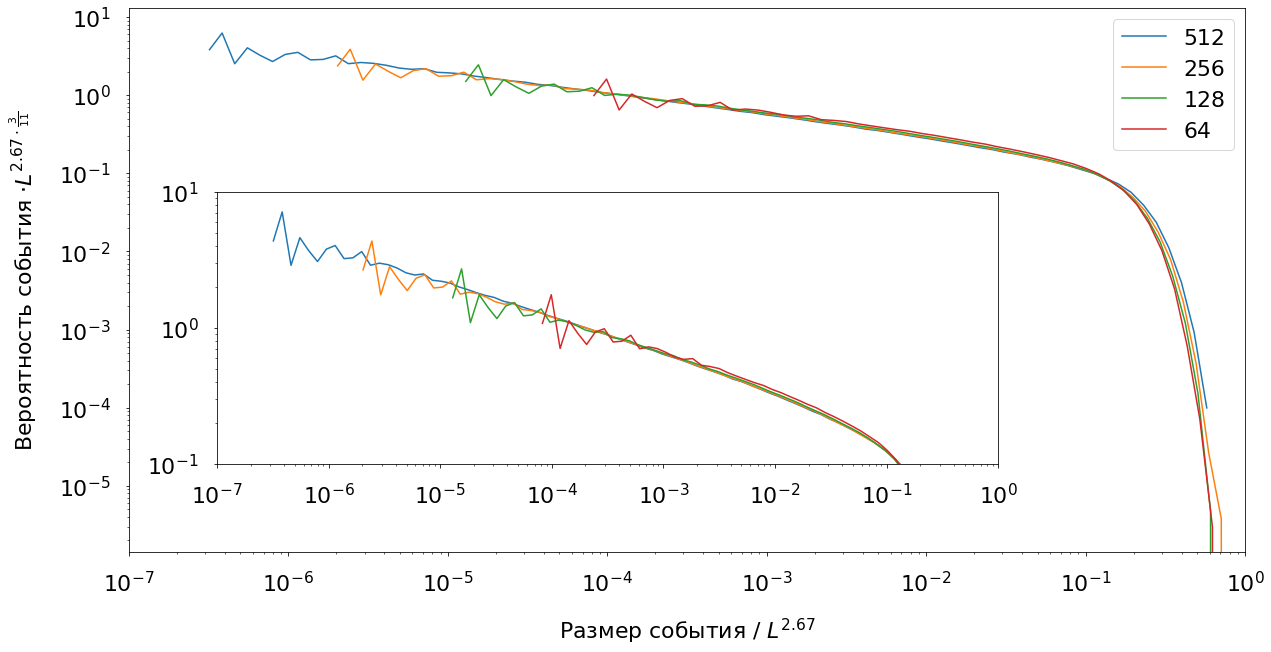
\includegraphics[width=\textwidth]{manna_distribution_267}
	\caption{Распределение событий в модели Манна с нормировкой $\gamma=2.67$}
\end{figure}

\begin{figure}[h]
	\centering
	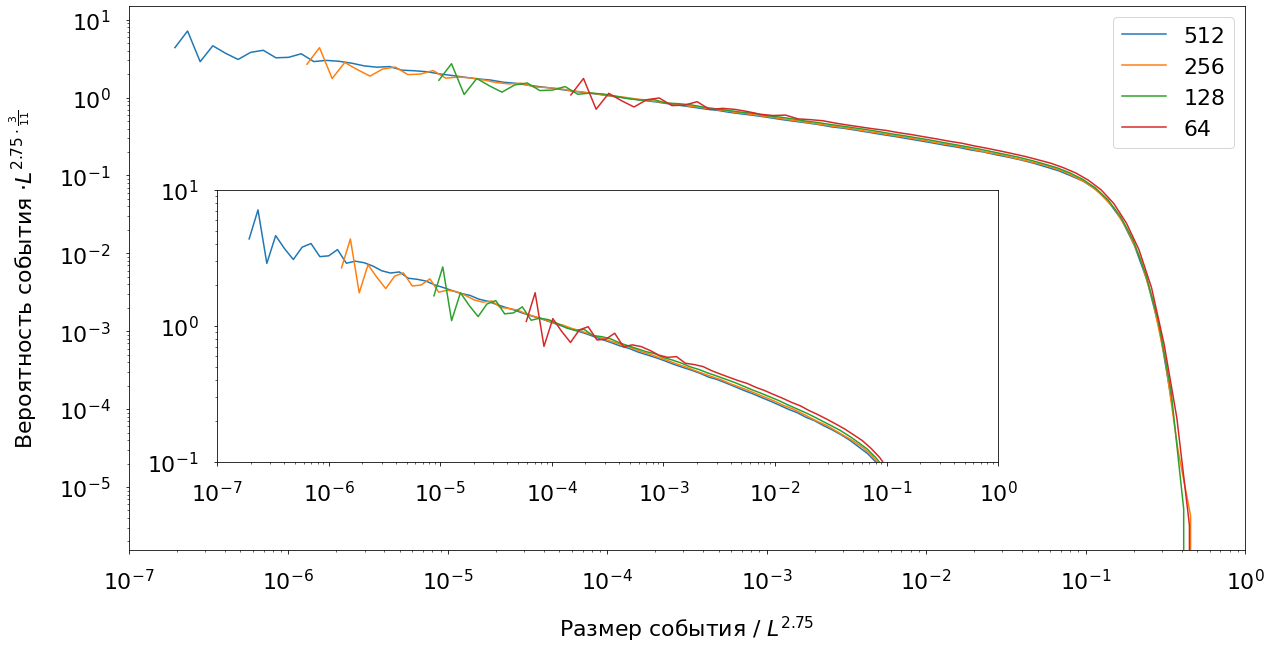
\includegraphics[width=\textwidth]{manna_distribution_275}
	\caption{Распределение событий в модели Манна с нормировкой $\gamma=2.75$}
\end{figure}